%!TEX root = ../main.tex

\section{Experimental Results}
\label{sec:results}

\subsection{State-Control Results}
Using the formulation of the problem above, \textrm{GPOPS-II} is able to find an optimal solution in a reasonable amount of time (minutes) for a small number of gates (approximately 10).
In \cref{fig:optimized_states}, we show the optimized states for the 6-gate racetrack in \cref{fig:optimizedz_trajectory}.

\begin{figure}[htbp]
  \centering
  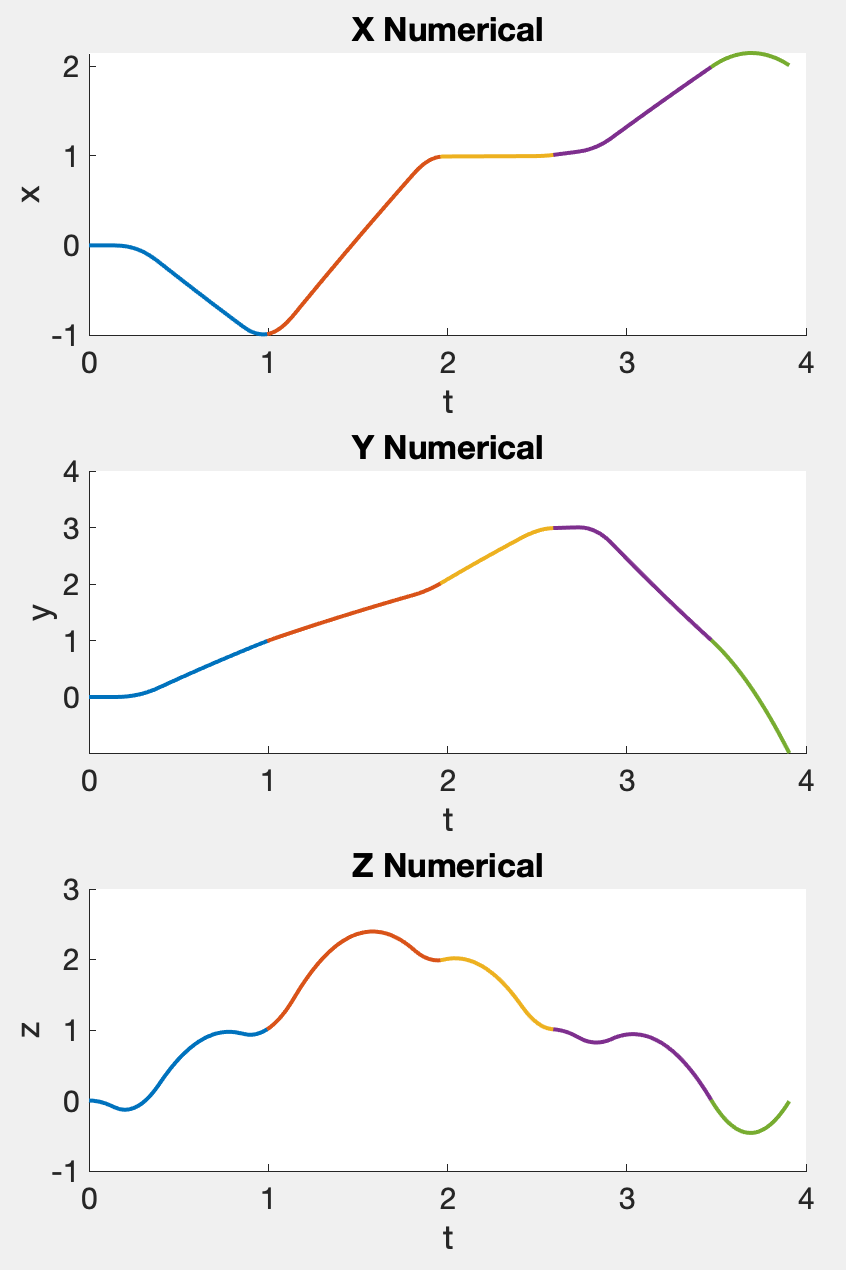
\includegraphics[width=1.0\columnwidth]{img/position.png}
  \caption{Optimized drone positions for the 6-gate environment in \cref{fig:optimized_trajectory}}.
  \label{fig:optimized_position}
\end{figure}

\begin{figure}[htbp]
  \centering
  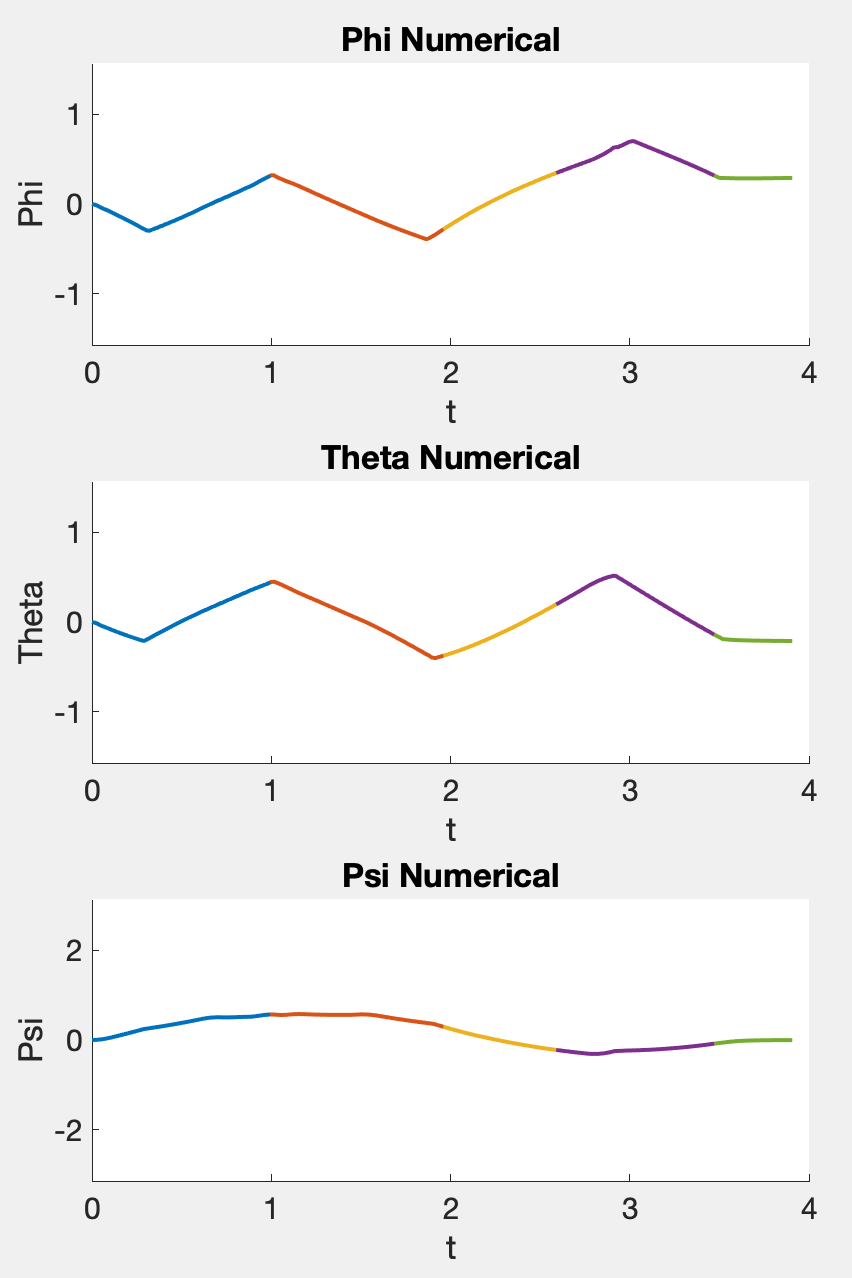
\includegraphics[width=1.0\columnwidth]{img/orientation.png}
  \caption{Optimized drone orientations for the 6-gate environment in \cref{fig:optimized_trajectory}}.
  \label{fig:optimized_orientation}
\end{figure}

\begin{figure}[htbp]
  \centering
  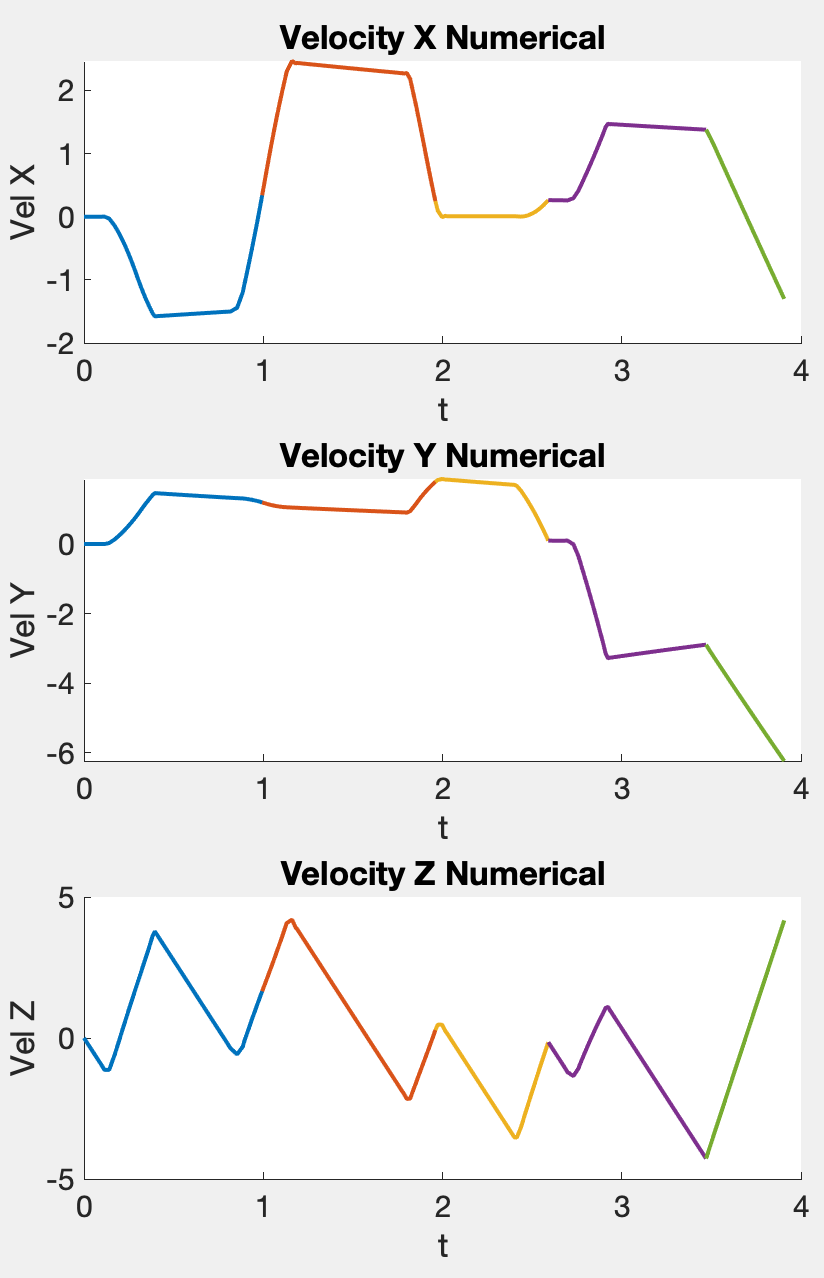
\includegraphics[width=1.0\columnwidth]{img/velocities.png}
  \caption{Optimized drone velocities for the 6-gate environment in \cref{fig:optimized_trajectory}}.
  \label{fig:optimized_velocities}
\end{figure}

\begin{figure}[htbp]
  \centering
  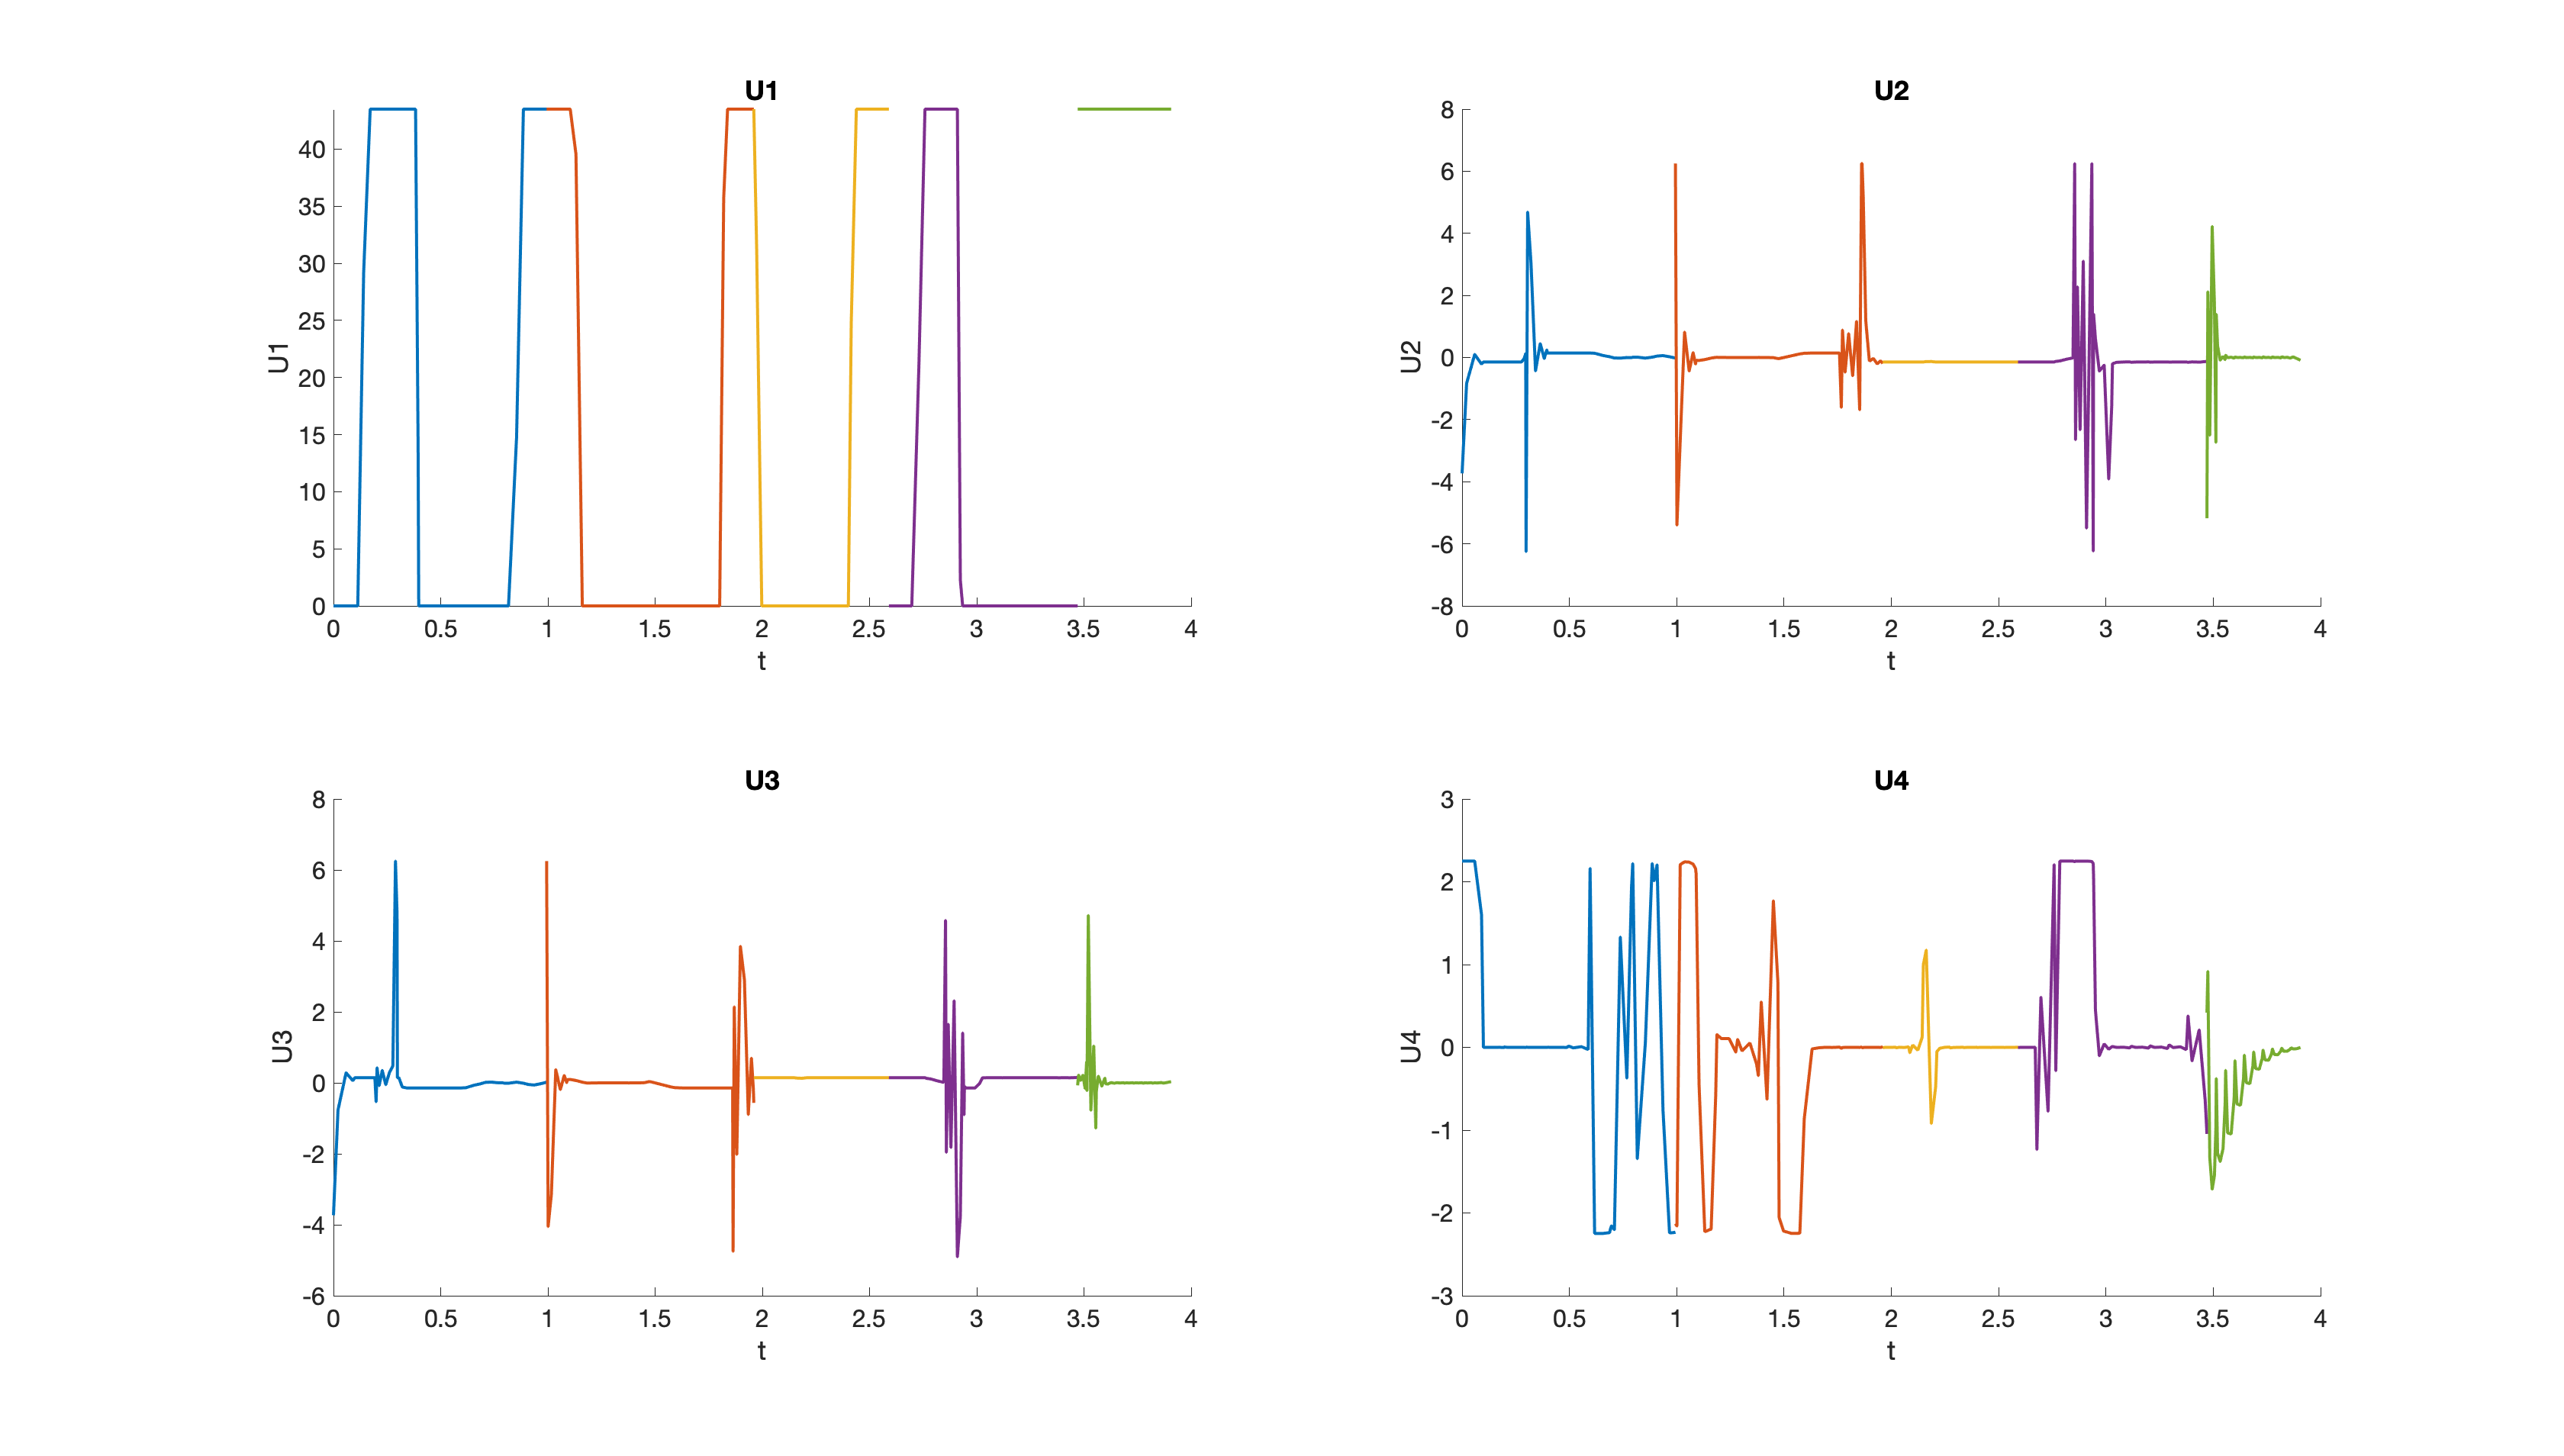
\includegraphics[width=1.0\textwidth]{img/controls.png}
  \caption{Optimized drone states for the 6-gate environment in \cref{fig:optimized_trajectory}}.
  \label{fig:optimized_controls}
\end{figure}

\begin{figure}[htbp]
  \centering
  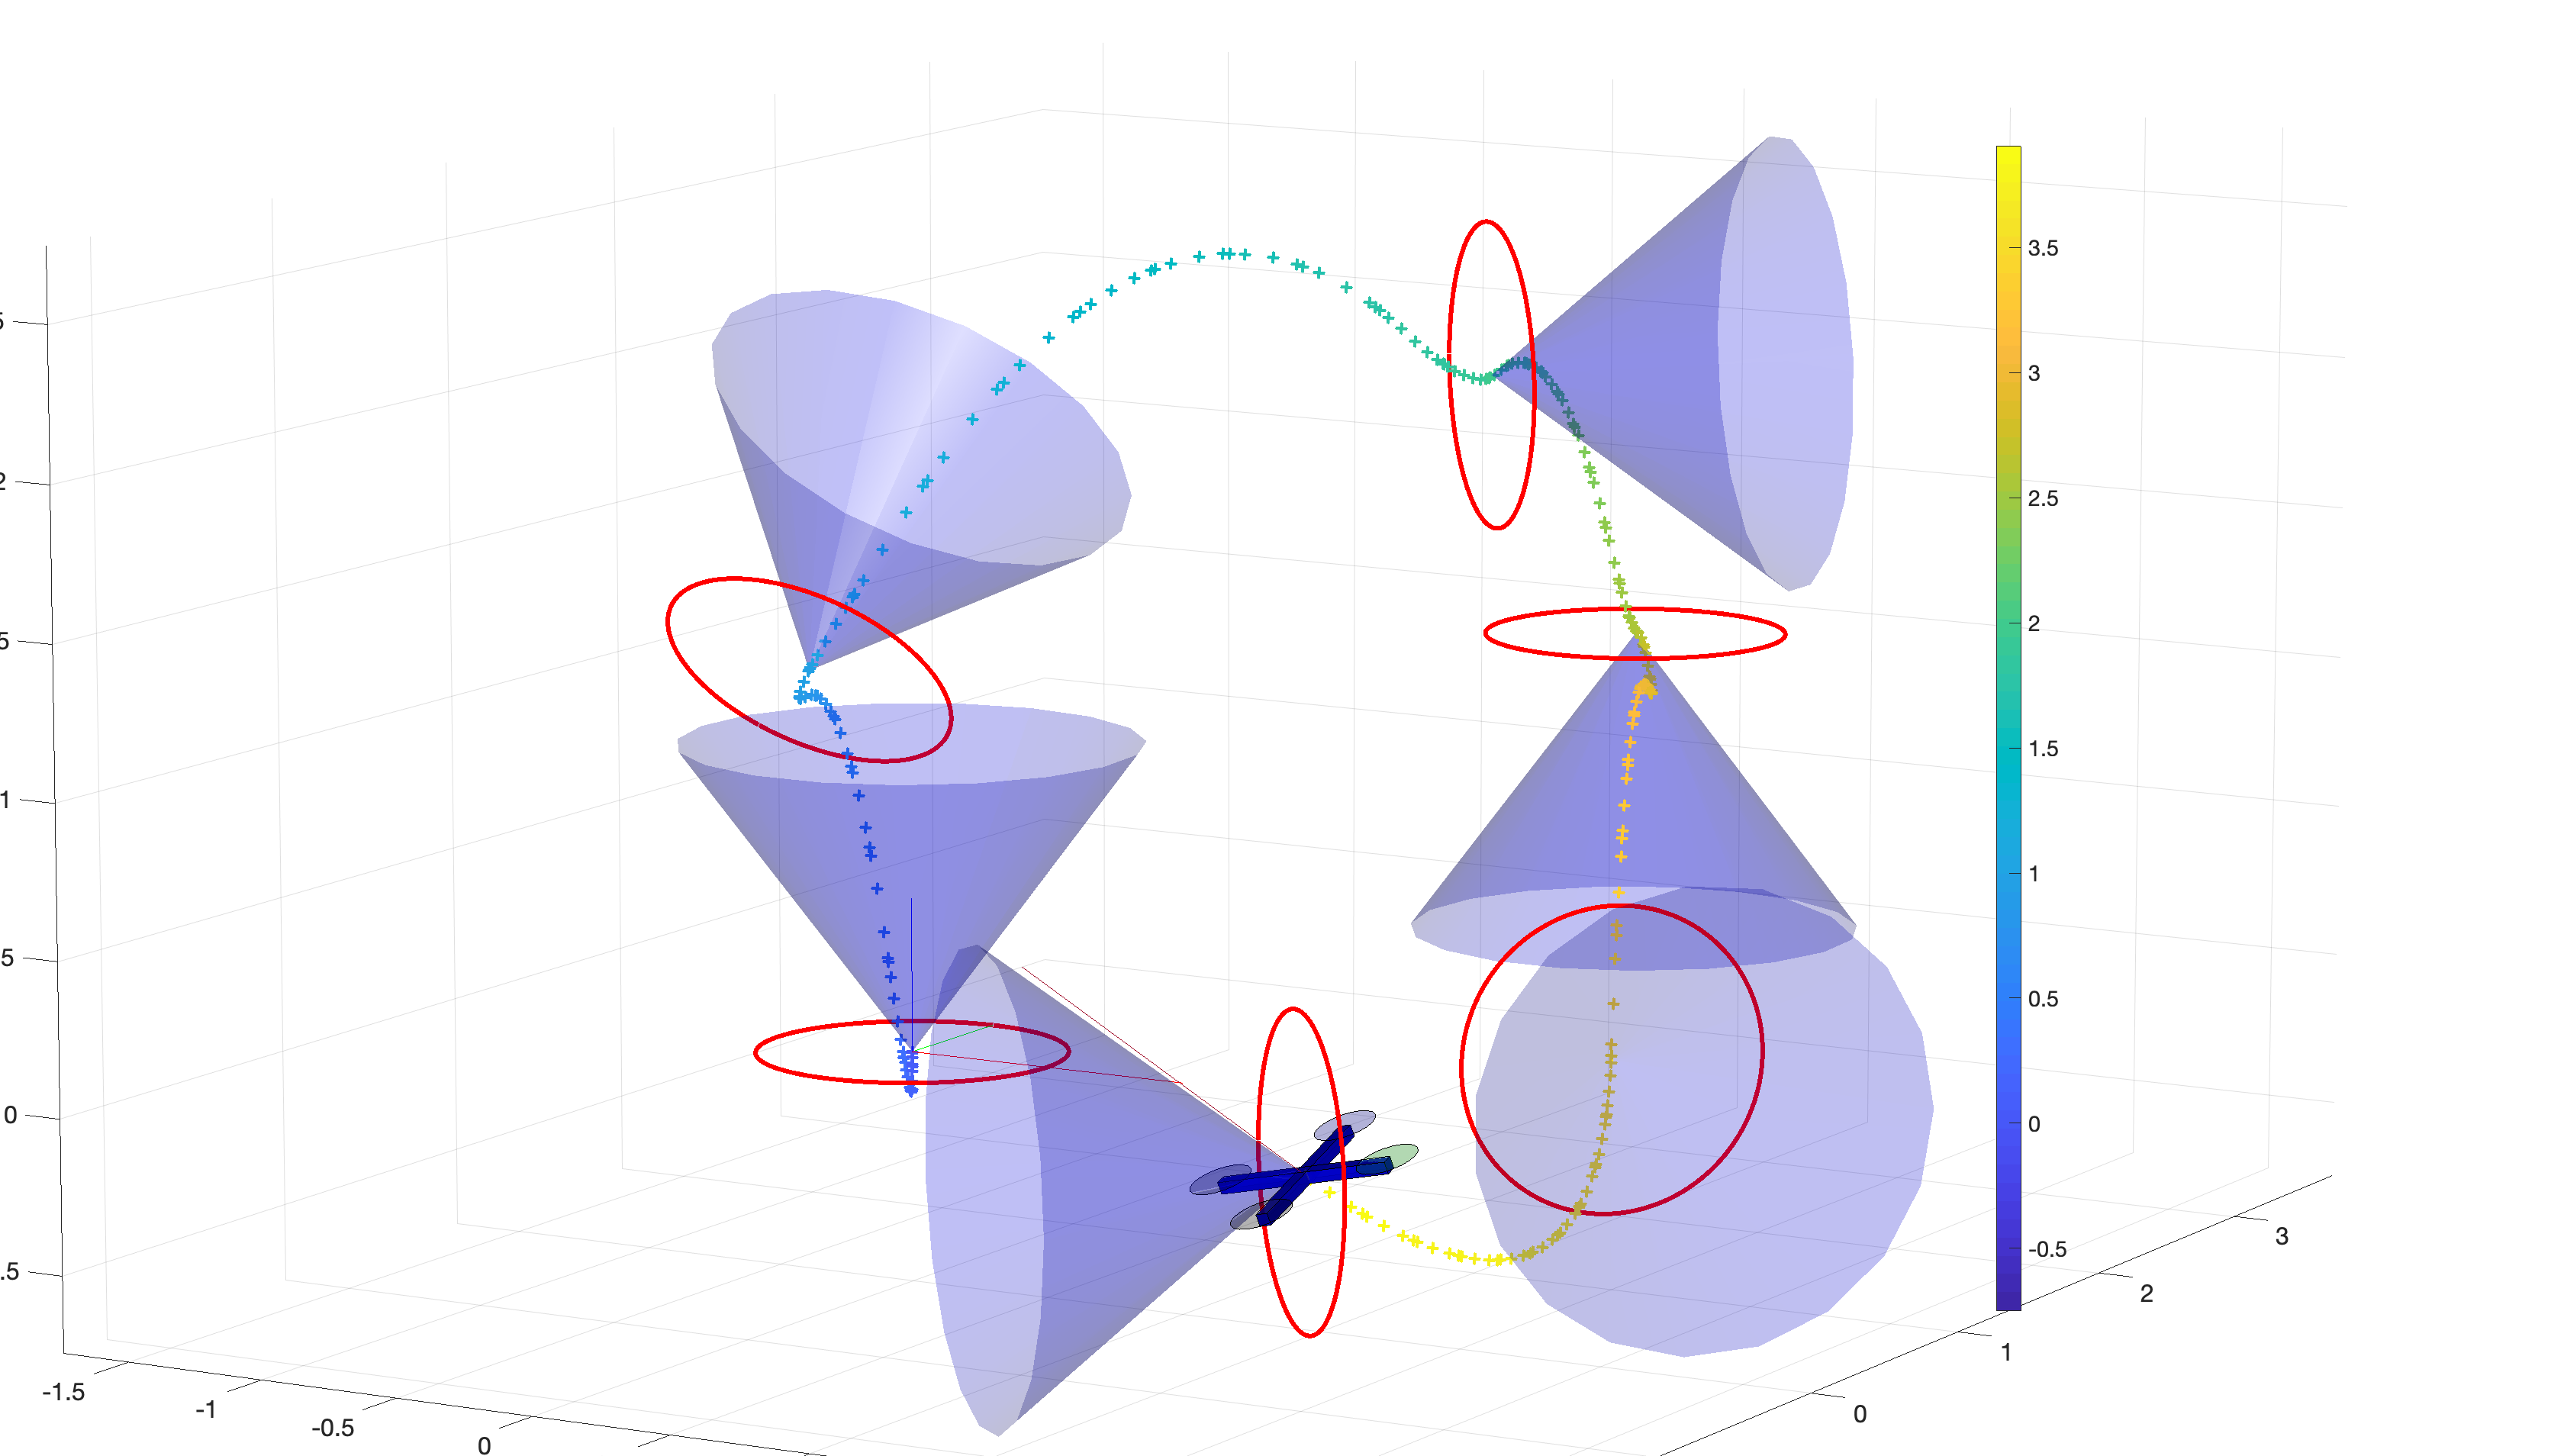
\includegraphics[width=0.8\textwidth, trim=700 0 0 0, clip]{img/DroneRaceTrajectoryOptWCones.png}
  \caption{6-gate drone racetrack with conic velocity constraints to ensure proper traversal of gates.}
  \label{fig:optimized_controls}
\end{figure}

\subsection{Modelling Limits and Extensions}